

%\begin{wrapfigure}[0.5]{R}{0.5\textwidth}
\begin{figure*}[t]\centering%
	%\scalebox{0.9}{\small\input{pics/diagram-20220513}}%overallApproach}}
	%\vspace*{-0.3cm}
	\centering
	%	\hspace{-0.9cm}
	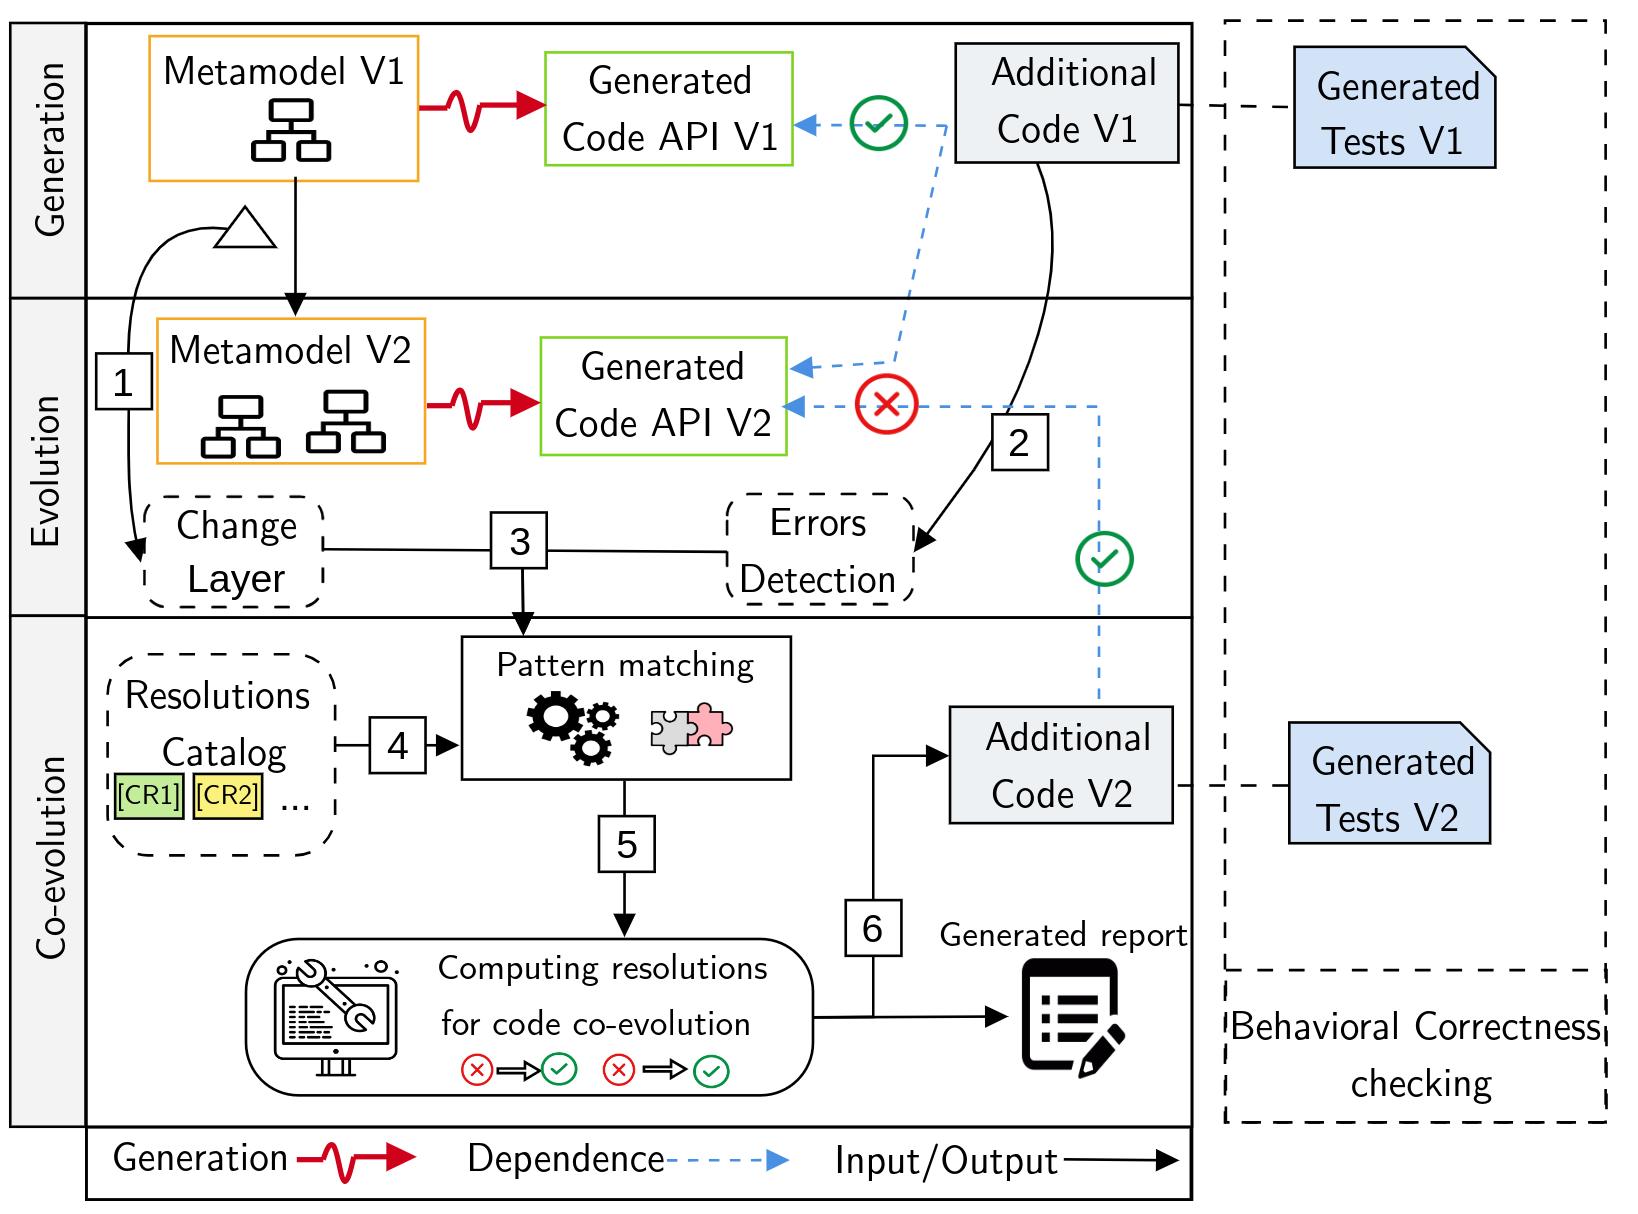
\includegraphics[width=0.8\textwidth]{./pics/chapter1pics/ApproachV5.png}
	\caption{Overall approach for metamodel and code co-evolution}
	\label{fig:overallapproach}
	%\vspace{-1em}
	\vspace{-1em}
\end{figure*}
%\end{wrapfigure}
\section{Change detection}
\label{sec: ap1_changedetection}

\section{Approach}\label{approach}

This section presents the overall approach of our automated co-evolution of code with evolving metamodels,  instantiating on the Ecore technological space. First, we give an overview of the approach and specify the metamodel evolution changes we consider. 
%
Then, we present how we retrieve the resulting errors due to metamodel evolution, followed by the regeneration of the code API. 
After that, we present the pattern matching process, which is an important part of our fully automatic co-evolution approach, before discussing the resolutions of the code errors. 

\subsection{Overview}
\label{Overview}

Figure~\ref{fig:overallapproach} depicts the overall steps for the automatic co-evolution of the metamodel and code, with horizontally separated parts defining chronological order from the top to the bottom.
%\\
After the generation step (the upper part of Figure~\ref{fig:overallapproach}), the evolution of the Ecore metamodel will cause errors in the additional Java code that depends on the API of the newly generated code (the middle part of Figure~\ref{fig:overallapproach}). We take as input the evolution changes of the metamodel between the two versions of this metamodel {\small\boxed{1}}. Then, we parse the additional code  {\small\boxed{2}} to retrieve the list of errors. 
After that, we get to the bottom part of Figure~\ref{fig:overallapproach}, both the list of metamodel changes and the list of errors are used as inputs for the pattern matching step {\small\boxed{3}}. It analyzes the structure of the error to match it with its impacting metamodel change and decides which resolution to apply for the error co-evolution {\small\boxed{4}}. The metamodel changes provide the ingredients and necessary information that are used for the co-evolution.  
At the end of the automatic co-evolution, we obtain a new co-evolved additional code {\small\boxed{5}}. 
In addition to the automatic co-evolution, we generate test cases before and after co-evolution to highlight its possible effect. In fact, many research papers rely on the use of tests to check the behavior of the code during its evolution. For example, Godefroid et al.~\cite{10.1145/3395363.3397374} uses tests to find regressions in different versions of REST APIs. In particular, Lamothe et al.~\cite{9079197},test ~\cite{10.1145/3387905.3388608} use tests to validate the evolution of the client code after Android API migration. We apply a similar method to check the effect of the co-evolution. \cite{10.5555/2486788.2486855}
Finally, during the co-evolution process, we generate a report linking the applied resolutions for each code error with its impacting metamodel change. If needed, this can help developers in understanding the performed co-evolution, since we fully automate it.
%\todo{refs behavioral check et papier android : to check}
%\DK{we see later if we add the story of generated tests after co-evolution}
